\documentclass[journal]{IEEEtran}
\usepackage[T1]{fontenc}
\usepackage[utf8]{inputenc}
\usepackage{amsmath,amssymb,graphicx,booktabs,array,tabularx}
\usepackage[caption=false,font=footnotesize]{subfig}
\usepackage{cite}
\usepackage[hidelinks]{hyperref}
\usepackage{url}
\usepackage{tikz}
\usetikzlibrary{arrows.meta,positioning}
\graphicspath{{figures/}}
\newcommand{\supp}[1]{Supplementary Section~S#1}
\newcommand{\op}{\mathrm{op}}
\newcommand{\refcase}{\mathrm{ref}}
\allowdisplaybreaks
\title{Characterisation and Quantification of Data Centre Flexibility for Power System Support}
\author{James Day, Mehmet T\"urker Takci, and Meysam Qadrdan\thanks{The authors are with Cardiff University, Queen's Buildings, The Parade, Cardiff CF24 3AA, United Kingdom. Corresponding author: James Day (DayJa1@cardiff.ac.uk).}}
\begin{document}
\maketitle
\begin{abstract}
Data centres can adjust electricity demand through workload scheduling, electrical storage and cooling control, but the flexibility available at the grid connection depends on how these resources interact. This paper presents an integrated model of IT workloads, uninterruptible power supply (UPS) batteries, cooling dynamics and thermal energy storage to characterise feasible power deviations and their duration. The assessment preserves computational work, respects operating limits and requires recovery relative to the undisturbed operating trajectory. Component decomposition shows how the resources combine, compensate for one another and change roles with event timing. For a facility with 1 MW of rated IT power, a representative-day assessment demonstrates import reductions of 100 and 150 kW lasting six hours, while a 25 kW import increase reaches the twelve-hour assessment cap. At other start times, the same requested reduction is supplied by a different combination of assets. A full year of linked daily optimisation provides the operating reference and evaluates electricity-cost savings under observed Great Britain reference prices. Coordinated operation reduces annual cost by 5.05\%, although electricity use and peak import increase. Enlarging UPS energy capacity from 600 to 900 kWh adds approximately GBP~2,481 in annual savings, enabling a conditional break-even investment assessment. The results establish the importance of describing data-centre flexibility through its magnitude, duration, operating state and recovery requirements, rather than installed capacity alone.
\end{abstract}
\begin{IEEEkeywords}
Data centres, demand-side flexibility, workload scheduling, thermal energy storage, uninterruptible power supply.
\end{IEEEkeywords}
\section{Introduction}
\label{sec:introduction}
\IEEEPARstart{D}{ata} centres are large electricity consumers whose internal operating choices can also provide flexibility to the power system. Their computing equipment, backup batteries and cooling infrastructure offer different ways to change demand, but these resources serve a common purpose: maintaining the facility's computational service. Assessing their flexibility therefore requires more than identifying spare electrical capacity. It requires establishing how much the facility can change its grid demand, for how long, and what must happen afterwards to restore its operating condition.

The significance of this question is increasing with the scale and concentration of digital infrastructure. In its 2025 \emph{Energy and AI} report, the International Energy Agency estimated that data centres consumed 415 TWh in 2024 and projected approximately 945 TWh by 2030 in its base case~\cite{iea_energy_ai}. Alongside this demand growth, increasing renewable generation strengthens the need to adjust electricity consumption to changing supply conditions. The geographical concentration of data centres makes their local demand profiles important as well as their aggregate energy use. Flexible operation could help accommodate these loads, provided that the response available from a facility can be described in terms useful to a system operator.

Data-centre flexibility has both an operational and an economic dimension. Work can be moved between permitted execution times, batteries can exchange energy with the internal electrical system, and cooling can use stored thermal energy or limited temperature variation. Such actions may reduce electricity expenditure or change demand in response to a grid request. However, a schedule that is attractive under electricity prices does not necessarily leave every resource ready to deliver an additional response. A charged battery, available computing capacity and a favourable thermal state cannot be assumed to coincide. The operating trajectory from which a request begins is therefore part of the definition of available flexibility.

Throughout this paper, \emph{upward flexibility} means a reduction in electricity import, supporting the system when demand must fall relative to supply. \emph{Downward flexibility} means an increase in import. Requested deviations are signed from the consumer's perspective: negative for reduced import and positive for increased import. The study characterises their feasible duration and the contributions of internal resources. It does not assume that the facility exports electricity or that a response lasting several hours establishes eligibility for a particular frequency-response product.

\subsection{Data-centre architecture}
\label{sec:architecture}
A data centre combines IT equipment with the electrical and thermal infrastructure needed to sustain it. Figure~\ref{fig:architecture} shows the system considered here. The uninterruptible power supply (UPS) supports continuity of electricity supply to the IT load. A chiller supplies the computer room air conditioning (CRAC) system and can also charge thermal energy storage (TES), allowing cooling production and cooling delivery to occur at different times. Thermal mass in the equipment and air adds a further dependence on previous operating decisions.

\begin{figure}[t]
\centering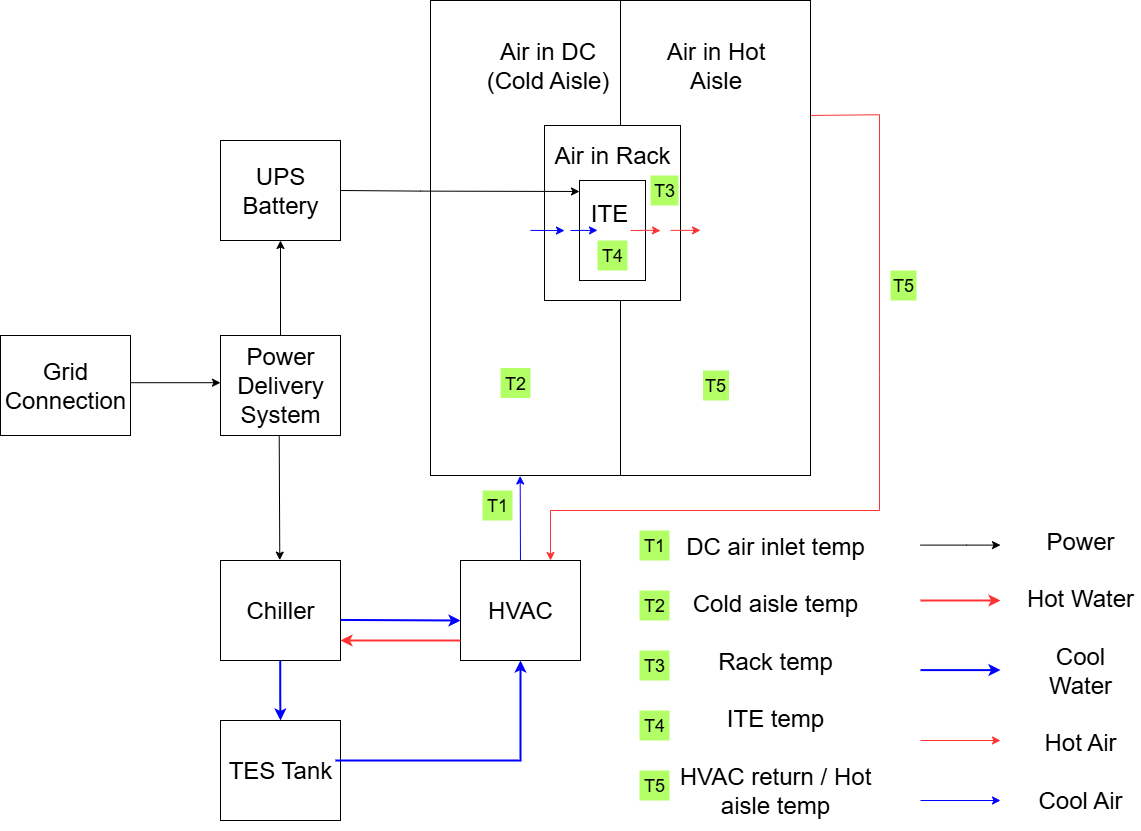
\includegraphics[width=\columnwidth]{Figure_1.png}
\caption{Data-centre architecture: IT demand, UPS storage and the coupled chiller, CRAC and TES system.}
\label{fig:architecture}
\end{figure}

These resources interact through both energy flows and operating constraints. Deferring computation reduces IT electricity demand and changes the heat that cooling must remove. TES discharge can reduce direct chiller electricity, while charging the store competes with immediate cooling for chiller capacity. UPS discharge can support IT execution without drawing the same power from the grid. Consequently, one resource can compensate while another completes deferred work or restores its state. Assessing assets independently can miss these compensating actions, or assign the same limited headroom to more than one service.

\subsection{Workloads and the questions addressed}
Computational tasks differ in their tolerance of delay. Interactive services generally require prompt execution, whereas eligible batch tasks can be scheduled within agreed windows~\cite{Cao2022ApEn,Liu2024Access}. This distinction depends on the application and its service-level agreement (SLA), rather than being a fixed property of all workloads of a given type. The model therefore treats workload flexibility as an input: an assumed share of arriving work can be rescheduled within specified limits, and the remainder executes at arrival. It preserves computational work and the modelled timing constraints; it does not represent all aspects of application performance.

Two questions guide the analysis. First, what combinations of power deviation and duration can the integrated facility deliver, and which resources supply them? Second, what electricity-cost savings arise from exploiting its operational flexibility over a full year, and how do those savings change with resource assumptions? The first question concerns physical capability. The second concerns economic operation under the modelled price signal. The annual schedule connects the two by providing the operating state from which additional grid deviations are assessed.

The paper makes three contributions. It presents an integrated representation of workload timing, UPS operation and cooling/TES that retains the couplings relevant to facility-level flexibility. It uses this representation to characterise state-dependent power deviations with post-event recovery, and to explain their internal composition. Finally, it evaluates annual electricity-cost savings and resource sensitivities, using the UPS results to identify the additional investment that the incremental savings could support. The annual rolling procedure supplies the temporal coverage needed for this valuation; it is not proposed as a new optimisation algorithm.

Section~\ref{sec:literature} places these contributions in the literature. Section~\ref{sec:methodology} describes the integrated model and assessment, and Section~\ref{sec:case-study} defines the case study. Section~\ref{sec:results} presents the flexibility characteristics, annual economic results and design implications. Section~\ref{sec:conclusion} concludes.

\section{Literature Review}
\label{sec:literature}
Research on data-centre flexibility spans workload scheduling, electrical storage, cooling control and coordinated facility operation. These strands establish the potential of individual resources and the importance of managing their interactions. The remaining assessment question is how to express the resulting facility response in terms of a requested change at the grid connection, its duration and its consequences for subsequent operation.

IT workload is a principal source of controllable demand. Cao et al.~\cite{Cao2022ApEn} investigate the temporal shifting capability of periodic batch workloads using a data-driven flexibility assessment. The approach makes workload characteristics central to the available response rather than treating the entire IT load as freely dispatchable. Misaghian et al.~\cite{Misaghian2023TIA} assess carbon-aware flexibility measures using machine learning, while Radovanovi\'c et al.~\cite{radovanovic2022carbon} describe carbon-aware computing that shifts eligible work in response to forecast grid conditions. These studies demonstrate the value of distinguishing work arrival from execution. They also show why flexibility depends on which tasks may move and which obligations must be met, not simply on the level of IT demand.

UPS batteries provide a complementary form of flexibility. Their power exchange can change without rescheduling the computational task being supplied. Alaper\"a et al.~\cite{alapera2018data} examine data centres as a source of dynamic flexibility, and subsequent pilot work investigates fast frequency response from a UPS system~\cite{alapera2019fast}. Such applications motivate the use of existing electrical storage for services beyond backup. They do not remove the need to reserve energy for the UPS's primary role or to consider conversion losses and battery ageing. A conventional storage formulation is appropriate when the research question concerns the battery's interaction with the rest of the facility rather than a new representation of battery physics.

Cooling flexibility is linked to heat production and to the thermal state of the facility. Cupelli et al.~\cite{cupelli2018data} develop a data-centre control framework for demand response using models of the coupled subsystems. Fu et al.~\cite{Fu2020ApEn} investigate coordinated IT and cooling control for frequency regulation. Thermal storage extends these opportunities by allowing cooling to be produced before it is needed, although its usefulness remains bounded by storage energy, charge and discharge rates, and the available chiller capacity. Work on data-centre heat recovery and short-term thermal storage also illustrates the importance of distinguishing the timing of thermal production and demand~\cite{du2025new}. The present study concerns cooling within the facility, rather than a district-heating export system.

Integrated operation is thus an established research direction. Cioara et al.~\cite{cioara2018optimized} consider flexibility management for data-centre participation in demand-response programmes, and Xu et al.~\cite{Xu2023SPIE} assess demand-response potential across multiple flexible resources. Cupelli et al.~\cite{cupelli2018data} are particularly relevant because the coupling between IT demand, electrical storage and thermal dynamics is already central to their control framework. The contribution sought here is therefore not the first combination of those resources. It is an explicit assessment of the power deviations and durations that their coordinated operation can sustain from a specified operating state, together with an account of how the components deliver the response and recover afterwards.

A scheduled operating profile and a flexibility envelope answer different questions. Cost or carbon optimisation identifies a preferred trajectory under its objective. A flexibility assessment asks which departures from that trajectory remain feasible. In a storage- and workload-constrained facility, feasibility during an event is insufficient if the response leaves depleted stores, excessive temperatures or additional unfinished work beyond the assessment window. Recovery conditions make these consequences part of the service definition. They also expose why the same requested grid deviation can require different internal actions at different times.

This study combines that duration-oriented assessment with annual economic evaluation. A single daily electricity-price profile can illustrate scheduling behaviour, but cannot establish the annual saving associated with repeated operation. Linked daily optimisation supplies that broader economic evidence while preserving the operating state used by the event assessment. The analysis retains the distinction between electricity-cost savings and grid-service revenues: the former are evaluated over the year, whereas the latter would require market-specific prices, availability requirements and delivery rules beyond the physical capability assessment conducted here.

\section{Methodology}
\label{sec:methodology}
\subsection{System boundary and modelling approach}
The model represents the facility at its electricity meter, with IT demand, UPS power exchange, direct cooling, TES charging and a fixed auxiliary load inside the boundary. Its purpose is to retain the variables that determine flexibility: unfinished computational work, storage energy and facility temperatures. Aggregate modelling permits these variables to be coordinated without representing the placement of each task on a server or the airflow around each rack~\cite{barroso2018datacenter,dayarathna2015data}. The resulting feasible response is conditional on this level of abstraction and the adopted operating limits.

Let $t$ index intervals of length $\Delta t=0.25$ h. Powers and processing rates apply during an interval; stored energies and temperatures are defined at its boundaries. Electrical and thermal powers are expressed in kW and kW-th, respectively, and stored energy in kWh or kWh-th. With UPS discharge supplying IT behind the meter, grid import is
\begin{equation}
\begin{split}
P_t^{\mathrm{grid}}={}&P_t^{\mathrm{IT}}+P_t^{\mathrm{U,ch}}-P_t^{\mathrm{U,dis}}\\
&+P_t^{\mathrm{C}}+P_t^{\mathrm{T,ch}}+P^{\mathrm{aux}},
\end{split}
\label{eq:grid}
\end{equation}
where $P^{\mathrm{C}}$ is chiller electricity for direct CRAC cooling and $P^{\mathrm{T,ch}}$ is chiller electricity for charging TES. UPS discharge cannot exceed contemporaneous IT demand; the facility does not export electricity. This balance also provides the basis for attributing a grid response to its internal components.

Figure~\ref{fig:workflow} sets out the assessment. Reference operation provides the annual cost comparator. Coordinated operation enables workload shifting and storage, yielding both annual electricity costs and the operating trajectory from which grid events are tested. The computational sequence establishes this trajectory first, even though the results foreground flexibility characterisation.
\begin{figure*}[t]
\centering
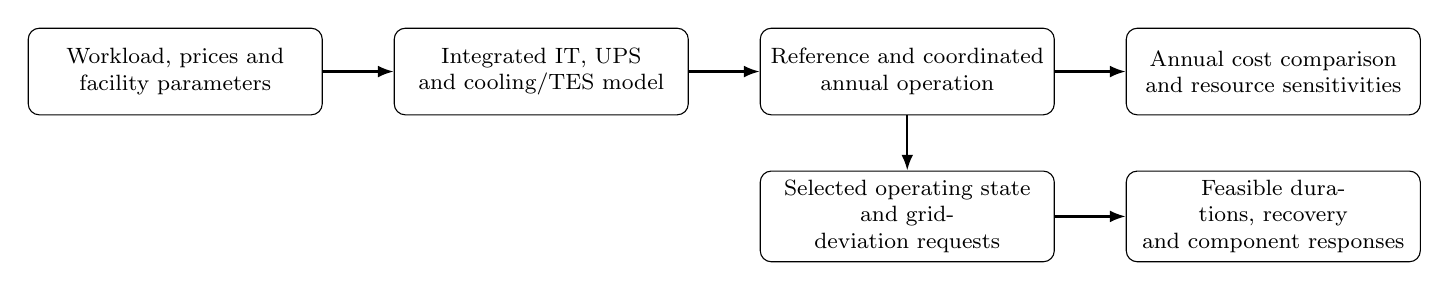
\begin{tikzpicture}[node distance=7mm and 9mm,box/.style={draw,rounded corners,align=center,font=\footnotesize,text width=35mm,minimum height=11mm},arr/.style={-{Latex[length=2mm]},thick}]
\node[box] (in) {Workload, prices and\\facility parameters};
\node[box,right=of in] (model) {Integrated IT, UPS\\and cooling/TES model};
\node[box,right=of model] (annual) {Reference and coordinated\\annual operation};
\node[box,right=of annual] (cost) {Annual cost comparison\\and resource sensitivities};
\node[box,below=of annual] (event) {Selected operating state\\and grid-deviation requests};
\node[box,right=of event] (flex) {Feasible durations, recovery\\and component responses};
\draw[arr] (in)--(model);\draw[arr] (model)--(annual);\draw[arr] (annual)--(cost);
\draw[arr] (annual)--(event);\draw[arr] (event)--(flex);
\end{tikzpicture}
\caption{Whole-study workflow. Annual operation supplies both economic results and the state used to characterise additional grid-facing flexibility.}
\label{fig:workflow}
\end{figure*}

\subsection{Workload scheduling and IT power}
Workload arrivals comprise an inflexible processing requirement and flexible cohorts. A cohort $c$ has arrival time $r_c$, CPU-hour requirement $a_c$, and a final eligible execution interval beginning at $\ell_c$. Its permitted set is $\mathcal W_c=\{t:r_c\leq t\leq\ell_c\}$. Assigning processing rate $u_{c,t}$ to that cohort gives the full-trajectory relations
\begin{equation}
\begin{gathered}
\sum_{t\in\mathcal W_c}u_{c,t}\Delta t=a_c,\qquad u_{c,t}\geq0,\\
u_t=u_t^{\mathrm{inflex}}+\sum_{c:t\in\mathcal W_c}u_{c,t}\leq1.
\end{gathered}
\label{eq:work}
\end{equation}
Only eligible work can be shifted, and it cannot execute before arrival. The classes permit final execution-interval starts 0.5, 1, 2 or 3 h after arrival. This is an interval-based deferral convention: processing in the final permitted interval finishes at its closing boundary. The exact indexing and the treatment of cohorts extending beyond an individual optimisation horizon are given in \supp{3}.

CPU-hours measure aggregate processor occupancy. They allow eligible computation to be distributed over different execution intervals while preserving the amount of work. This abstraction does not assume that all applications can be divided or accelerated arbitrarily; those properties are represented by the workload eligibility and timing assumptions. In particular, preserving computational work does not require electrical energy to be identical between schedules.

The analytic IT power relation is
\begin{equation}
f(u)=P^{\mathrm{IT}}_{\mathrm{idle}}+
(P^{\mathrm{IT}}_{\max}-P^{\mathrm{IT}}_{\mathrm{idle}})u^{1.32}.
\label{eq:power}
\end{equation}
It captures the increase in server power with utilisation~\cite{dayarathna2015data,v2015analysis}. Both reference and coordinated operation use the same four-segment piecewise-linear approximation $P_t^{\mathrm{IT}}=\widehat f(u_t)$. The optimisation is consequently a mixed-integer linear programme (MILP), rather than a direct nonlinear optimisation of Equation~\eqref{eq:power}. Breakpoints, approximation error and the logarithmic formulation are documented in \supp{3}.

\subsection{Electrical and thermal flexibility}
The UPS and TES shift electrical and cooling energy, respectively. Their boundary-state equations are
\begin{equation}
\begin{aligned}
E^{\mathrm{U}}_{t+1}&=E^{\mathrm{U}}_t+
\left(\eta_{\mathrm{U,ch}}P_t^{\mathrm{U,ch}}-
\frac{P_t^{\mathrm{U,dis}}}{\eta_{\mathrm{U,dis}}}\right)\Delta t,\\
E^{\mathrm{T}}_{t+1}&=E^{\mathrm{T}}_t+
\left(\eta_{\mathrm{T,ch}}Q_t^{\mathrm{T,ch}}-
\frac{Q_t^{\mathrm{T,dis}}}{\eta_{\mathrm{T,dis}}}\right)\Delta t.
\end{aligned}
\label{eq:stores}
\end{equation}
Each store has energy and charge/discharge power limits, with one binary mode variable preventing simultaneous charging and discharging. The UPS retains a reserve of 50\% of its modelled nameplate energy. Its available operational energy window is therefore half that capacity. No daily cyclic restoration is imposed: subsequent operation inherits the resulting state. Standing losses and ageing costs are excluded, while conversion losses are included through the efficiencies.

The chiller couples the two cooling paths:
\begin{equation}
\begin{gathered}
Q_t^{\mathrm{cool}}=\mathrm{COP}\,P_t^{\mathrm{C}}+Q_t^{\mathrm{T,dis}},\qquad
Q_t^{\mathrm{T,ch}}=\mathrm{COP}\,P_t^{\mathrm{T,ch}},\\
P_t^{\mathrm{C}}+P_t^{\mathrm{T,ch}}\leq P_{\max}^{\mathrm{chiller}}.
\end{gathered}
\label{eq:cooling}
\end{equation}
Charging TES uses capacity that could otherwise produce immediate cooling. Discharging TES supplies cooling without the corresponding contemporaneous chiller electricity. Its contribution at the meter is consequently mediated by the chiller loads, rather than appearing as an independent electrical injection.

IT electricity becomes heat in a four-node thermal model adapted from Cupelli et al.~\cite{cupelli2018data}. The states represent IT equipment, rack air, cold-aisle air and hot-aisle air. Backward-Euler updates retain their dynamics at the quarter-hour resolution. The full recursions, inlet-temperature relation and calibrated effective-airflow factor are in \supp{3}. Temperature limits apply throughout each horizon, including the recovery period.

The adopted model also constrains gross cooling provision by
\begin{equation}
P_t^{\mathrm{IT}}\leq Q_t^{\mathrm{cool}}\leq
\dot m c_p\bigl(T_{t+1}^{\mathrm{HA}}-T_{\min}^{\mathrm{CA}}\bigr).
\label{eq:coolbound}
\end{equation}
The lower bound is a conservative operating rule limiting reliance on heat accumulation; it is not asserted to be a universal requirement of thermal physics. The upper bound limits inlet cooling. These restrictions matter to the interpretation of thermal flexibility: the model allows temperature dynamics and TES operation, but does not credit unrestricted undercooling as an additional resource. Thus the thermal model describes an adopted operating envelope, rather than an unconstrained thermodynamic maximum.

\subsection{Power-deviation, duration and recovery assessment}
Let $P_t^{\op}$ denote grid import under coordinated operation. For an event starting at $t_0$ with duration $\tau$ and signed deviation $\Delta P$, the event schedule must satisfy
\begin{equation}
\left|P_t^{\mathrm{grid}}-(P_t^{\op}+\Delta P)\right|
\leq\epsilon_P,\quad t_0\leq t<t_0+\tau,
\label{eq:target}
\end{equation}
where $\epsilon_P=0.1$ kW. Each trial begins from the physical state and unfinished cohort ledger recorded at $t_0$. There is no pre-event optimisation to charge a store or accumulate work in anticipation of the request.

Recovery is assessed at $H=t_0+\tau+3$ h relative to the undisturbed coordinated trajectory. With $R_{c,H}$ denoting remaining work for cohort $c$, the requirements are
\begin{equation}
\begin{gathered}
E_H^{\mathrm{U}}\geq E_H^{\mathrm{U},\op},\qquad
E_H^{\mathrm{T}}\geq E_H^{\mathrm{T},\op},\\
|T_H^j-T_H^{j,\op}|\leq0.05^{\circ}\mathrm C,
\quad j\in\{\mathrm{IT,R,CA,HA}\},\\
R_{c,H}\leq R_{c,H}^{\op}+10^{-7}\ \mathrm{CPU\,h}.
\end{gathered}
\label{eq:recovery}
\end{equation}
Original workload execution windows remain in force. The grid target is released during recovery, allowing compensating consumption, but the event cannot leave less stored energy or additional unfinished work relative to the reference beyond the specified tolerances. Recovery therefore means satisfying these comparative conditions, not returning every state exactly to its pre-event value.

Candidate durations are multiples of 15 minutes, bounded by twelve hours and the end of the selected local day. The search first tests the assessment cap, then uses a logarithmic search and an adjacent-duration check. All reported positive durations have an accepted, audited feasible dispatch. An unresolved trial is not evidence of infeasibility. Because the recovery reference changes with $\tau$, adjacent checks alone do not establish global monotonicity of duration feasibility. Results are accordingly reported as \emph{certified feasible durations}, distinguishing cap-reaching cases and unresolved next steps; they are not asserted to be globally maximal durations in every cell. \supp{5} gives the search and status conventions.

Every event trial minimises signed electricity cost over its event and recovery window subject to the request. The component plots represent the accepted feasible solution to that objective; alternative allocations may exist. Subtracting the undisturbed schedule from Equation~\eqref{eq:grid} gives
\begin{equation}
\begin{split}
\Delta P_t^{\mathrm{grid}}={}&\Delta P_t^{\mathrm{IT}}+
\Delta P_t^{\mathrm{C}}+\Delta P_t^{\mathrm{T,ch}}\\
&+\Delta(P_t^{\mathrm{U,ch}}-P_t^{\mathrm{U,dis}}).
\end{split}
\label{eq:decomposition}
\end{equation}
The fixed auxiliary load cancels. Components may act in opposite directions, but their sum must track the request. This is a decomposition of dispatch, not an allocation of independent asset values.

\subsection{Annual economic evaluation}
For each local day $d$, the MILP minimises
\begin{equation}
\min\sum_{t\in\mathcal H_d}\pi_tP_t^{\mathrm{grid}}\Delta t/1000,
\label{eq:objective}
\end{equation}
where $\pi_t$ is the signed electricity reference price in GBP/MWh and $\mathcal H_d$ contains the local day and twelve look-ahead intervals. Only the local-day decisions are committed. UPS/TES energy, all four temperatures and unfinished cohorts pass to the next day, with each cohort retaining its original arrival and final eligible execution interval. Normal days contain 96 committed intervals; daylight-saving transitions contain 92 or 100. An absolute UTC timeline preserves continuous physical time.

Annual cost is the sum over committed 2025 intervals, with overlapping look-ahead intervals counted only when they become committed. Actual prices for the first three hours of 1 January 2026 provide the final continuation, which is excluded from 2025 settlement. No terminal energy credit is imposed. The annual saving is $C^{\refcase}-C^{\op}$, and its percentage is $100(C^{\refcase}-C^{\op})/C^{\refcase}$. Reference operation already optimises cooling; the comparison measures the further value of workload scheduling and storage coordination.

This retrospective calculation uses known inputs within each daily horizon. It evaluates operation through a full year, rather than extrapolating one selected day's saving, but it neither models forecast error nor solves one globally optimal year-long programme. Pyomo and HiGHS are used with a requested 0.1\% relative gap and a 300 s daily limit. Feasibility and accounting checks accompany the accepted solutions. The detailed handoff algorithm, terminal treatment and solver exceptions are in \supp{4} and \supp{7}.

\section{Case Study}
\label{sec:case-study}
\subsection{Facility and operating inputs}
The case study represents a stylised facility with 1 MW of rated IT power. This rating identifies the computational equipment scale; it is not a 1 MW grid-connection limit. Cooling, auxiliaries and UPS charging contribute additional import. Table~\ref{tab:parameters} lists the principal settings, and \supp{1} provides the complete parameter set.
\begin{table}[t]
\centering\caption{Principal case-study parameters.}
\label{tab:parameters}
\begin{tabular}{@{}lr@{}}\toprule
Parameter & Value\\\midrule
IT rated / idle power & 1,000 / 166.7 kW\\
UPS nameplate energy & 600 kWh\\
UPS operational energy range & 300--600 kWh\\
UPS charge / effective discharge limit & 270 / 1,000 kW\\
UPS charge / discharge efficiency & 0.82 / 0.92\\
TES energy / charge and discharge limits & 1,000 kWh-th / 300 kW-th\\
TES charge / discharge efficiency & 0.9 / 0.9\\
Chiller electrical limit / COP & 400 kW / 5\\
Fixed auxiliary demand & 53.095 kW\\
Structural grid-import limit & 1,723.095 kW\\
Outdoor temperature & $22^{\circ}$C\\
Cold-aisle / inlet-air bounds & 18--23 / 18--30$^{\circ}$C\\
Workload deferral classes & 0.5, 1, 2, 3 h\\\bottomrule
\end{tabular}
\end{table}

The daily workload profile is a modelling assumption informed by published workload and flexibility studies~\cite{Cao2022ApEn,6779441,Misaghian2023TIA,Liu2012PER}. It is not a measured trace of a particular facility. Flexible and inflexible utilisation are specified at quarter-hour resolution. The allocation of flexible arrivals among the four deferral classes is specified hourly, with each hourly distribution held constant over four consecutive quarter-hours. These profiles repeat by local clock time throughout the year. \supp{2} provides the 24 hourly tranche distributions and all 96 combined input rows, and distinguishes within-hour utilisation changes from constant hourly tranche shares. Workload composition is an assumption tested by sensitivity, not a general estimate of the fraction of all data-centre work that is shiftable.

The annual price signal is the 2025 Intermittent Market Reference Price (IMRP) published by the Low Carbon Contracts Company~\cite{lccc_imrp_actuals}. Each hourly Great Britain day-ahead reference price is assigned unchanged to four quarter-hour intervals. Negative observations retain their sign. IMRP is used as a wholesale reference signal; the objective does not contain network charges, capacity charges, levies or supplier margins. Fixed ambient temperature and COP isolate the scheduling interactions from seasonal changes in cooling efficiency. The auxiliary demand is also fixed and identical between cases. Its 53.095 kW value originates from a 7\% calibration against an earlier daily IT-plus-cooling load; it is not recalculated as a percentage of annual demand.

\subsection{Reference, coordinated and event cases}
Table~\ref{tab:cases} distinguishes the annual comparator from the operating trajectory used for event assessment. Both annual cases begin with 600 kWh in the UPS, 500 kWh in TES, and IT, rack, cold-aisle and hot-aisle temperatures of $(28.5,26,20,27)^{\circ}$C. Subsequent days inherit states rather than resetting them. Reference cooling is cost optimised within the same temperature limits as coordinated cooling; savings are therefore not attributed to introducing a different cooling-control benchmark.
\begin{table*}[t]
\centering\caption{Cases and their roles in the analysis.}
\label{tab:cases}
\begin{tabularx}{\textwidth}{@{}lXXX@{}}\toprule
Case & Workload and storage & Cooling and operating state & Output\\\midrule
Reference operation ($\refcase$) & All work executes at arrival; UPS and TES dispatch disabled & Cooling cost optimised; temperatures continuous between days & Annual cost comparator\\
Coordinated operation ($\op$) & Eligible work rescheduled; UPS and TES dispatch enabled & Same thermal model and bounds; all states and unfinished work carried forward & Annual cost and undisturbed event reference\\
Flexibility event & Same eligibility and equipment limits; an additional grid target is imposed & Begins from coordinated state; comparative recovery after the event & Feasible duration and component response\\\bottomrule
\end{tabularx}
\end{table*}

The event day is selected using the smallest standardised distance to annual daily price, demand, utilisation, cost and opening-state characteristics. Eligible days contain 96 intervals and precede the final three days of the year. The selected day is 22 September 2025. Its actual physical states and per-cohort execution record initialise each request; the full selection rule is in \supp{5}. Event starts are sampled hourly. Reduced-import requests range from 100 to 500 kW in 50 kW steps; increased-import requests are 25, 50 and 75 kW, giving 288 start-time/request pairs. These are the evaluated request ranges, not a claim that both directions have been explored over equal power ranges.

\subsection{Sensitivity and UPS investment screen}
The annual sensitivity changes flexible workload share, UPS energy capacity and TES energy capacity one at a time to 0.5, 0.75, 1.25 and 1.5 times the central setting. The shared central case completes each five-point curve. All settings use the full 365-day trajectory. Workload scaling transfers processing requirements between the flexible and inflexible pools while preserving total arrivals; flexible utilisation is capped by total available workload. Storage sensitivities hold power ratings fixed and preserve initial state-of-charge fractions. UPS reserve remains 50\% of the changed capacity. These are energy-capacity tests, not joint power-and-energy sizing studies.

For UPS enlargement, the relevant benefit is the additional saving relative to the 600 kWh coordinated case. A conditional investment screen converts that annual benefit into a break-even capital amount using the capital recovery factor~\cite{sam_crf}:
\begin{equation}
I_{\mathrm{BE}}(E)=\frac{C^{\op}(600)-C^{\op}(E)-O_{\mathrm{add}}}
{r(1+r)^n/[(1+r)^n-1]},
\label{eq:investment}
\end{equation}
where $r$ is the real discount rate, $n$ the assessment life and $O_{\mathrm{add}}$ additional annual non-electricity costs. The illustrative main comparison uses 8\% and ten years, with constant real benefits and no additional O\&M, ageing, replacement cost or residual value. These are transparent screening assumptions, not a forecast or a vendor price estimate. \supp{8} gives alternative rates and lives and explains the limitations of repeating a single-year saving.

\section{Results and Discussion}
\label{sec:results}
\subsection{Operating reference for the flexibility assessment}
The selected day's coordinated trajectory establishes what the facility would be doing before receiving an additional grid request. Figure~\ref{fig:day} shows the corresponding grid import and workload execution. Computation moves between eligible intervals, with lower import around some price peaks and higher import when work is completed or storage is charged. The arrival profile remains unchanged: scheduling alters execution, not the computational demand presented to the facility.

\begin{figure*}[t]
\centering
\subfloat[Grid import and electricity reference price.]{
\includegraphics[width=0.49\textwidth]{Figure_4a.png}}\hfill
\subfloat[Workload arrival and execution.]{
\includegraphics[width=0.49\textwidth]{Figure_4b.png}}
\caption{Reference and coordinated operation on 22 September 2025. The figures' ``baseline'' denotes reference operation; the coordinated trajectory is the undisturbed reference for the subsequent event assessment. Opening states are inherited from the preceding day.}
\label{fig:day}
\end{figure*}

The scheduling pattern reflects more than the instantaneous price. Work already deferred has a shrinking execution window; charging is limited by power ratings and available capacity; and changes in IT execution alter cooling requirements. Thus neither installed capacity nor the local price alone determines the response still available at a given time. The heatmap and component results below assess that remaining capability from the actual coordinated trajectory.

\subsection{Magnitude, duration and direction of response}
Figure~\ref{fig:envelope} reports certified feasible duration for each requested deviation and start time. Reduced-import requests of 100 and 150 kW are sustained for six hours from noon. This corresponds to reductions of 10\% and 15\% of rated IT power, while the actual target is defined at the whole-facility meter. A 25 kW increased-import request reaches the twelve-hour assessment cap at 03:00 and at 10:00, 11:00 and 12:00. These cap-reaching results establish twelve-hour feasibility under the recovery conditions; they do not establish an intrinsic upper limit of twelve hours.

\begin{figure*}[t]
\centering
\includegraphics[width=\textwidth]{Figure_6.png}
\caption{Certified feasible duration on 22 September 2025. Negative deviations reduce import; positive deviations increase it. Blank cells mean that no positive duration was certified by the search. A plus sign marks an unresolved next 15-minute trial. Durations reaching twelve hours or the remaining local-day length are assessment-capped. Other unmarked positive cells have an adjacent tested boundary; the search does not establish global maximality for every cell.}
\label{fig:envelope}
\end{figure*}

The dominant feature is the dependence on operating time. A 100 kW reduction lasts 1.25 h from 06:00 and 6 h from noon, despite unchanged equipment ratings. The storage state, unfinished workload and thermal trajectory differ between these starts. Those conditions determine both what can be curtailed during the event and whether its consequences can be recovered afterwards. The absence of a certified response at another time should therefore not be interpreted as the absence of installed flexible equipment.

Within the tested grid, larger requested magnitudes generally have shorter certified durations, with plateaus where different magnitudes reach the same duration. The two directions also differ. Small import increases can be assembled over long periods by executing eligible work earlier than in the coordinated schedule and by changing storage and cooling operation. Import reduction depends on being able to defer execution, reduce chiller demand or supply IT from the UPS. Since the tested increased-import requests are substantially smaller than the reduced-import requests, the comparison does not isolate direction from magnitude. It demonstrates the capabilities evaluated here, rather than a complete symmetric power range.

Two assessment boundaries are important when reading the figure. First, an event cannot extend beyond the selected local day, although recovery may continue for three hours afterwards. The declining late-day durations consequently reflect this assessment limit as well as physical capability. Second, thirteen cells retain a plus sign because the next candidate duration remained unresolved. For example, the 25 kW increase at 06:00 is feasible for at least 11.25 h, and the 50 kW increase for at least 8.75 h. A solver timeout cannot establish that a longer response is impossible.

The reported durations include the requirement to recover relative to undisturbed operation. This prevents a response from appearing feasible merely because it leaves storage depleted or additional work outstanding beyond the comparison window. Nevertheless, the heatmap remains a state-conditioned illustration from one day. It does not indicate how frequently these durations would be available during the year, or the dependable capacity that could be offered into a particular market.

\subsection{How internal resources deliver the grid response}
The component results explain why a single facility-level deviation can conceal very different operating actions. Figures~\ref{fig:reduction} and \ref{fig:increase} show changes from the coordinated trajectory, with positive and negative component changes summed according to Equation~\eqref{eq:decomposition}. Their interpretation is electrical: TES is represented through changes in chiller electricity, and UPS through net charging minus discharging. The allocation is one accepted cost-minimising dispatch under the request constraints, rather than a unique division of the response among assets.

\begin{figure*}[t]
\centering
\includegraphics[width=\textwidth]{Figure_7.png}
\caption{Component changes for selected reduced-import events. The dashed line identifies the requested deviation during the event; the target is not imposed in the grey post-event region. Recovery is verified by terminal constraints, rather than fully displayed in these panels.}
\label{fig:reduction}
\end{figure*}
\begin{figure*}[t]
\centering
\includegraphics[width=\textwidth]{Figure_8.png}
\caption{Component changes for selected increased-import events. Opposing component actions can be larger than the net requested deviation. Grey regions, where present, follow the certified event; the target is released during recovery.}
\label{fig:increase}
\end{figure*}

The reduced-import cases provide a particularly clear comparison. At 06:00, the selected 100 and 200 kW reductions are delivered entirely through additional UPS discharge for 1.25 h; IT and chiller demand remain at the coordinated values. At 15:00, both requested reductions are sustained for 3 h, but the response is supplied mainly by deferred IT execution and reduced direct cooling. TES is full and idle in the undisturbed trajectory at that start, so there is no TES charging to curtail. The 200 kW case is delivered by IT and cooling alone; the 100 kW case includes only a single 37 kW UPS-discharge interval. Installed energy is therefore not a reliable guide to which resource will participate in an event.

The IT--cooling interaction is visible in the afternoon cases. Moving computation changes both its direct electrical demand and the timing of heat generation. Cooling consequently contributes to the metered reduction alongside IT. A workload-only power model would omit that thermal consequence, while a cooling model driven by an unchanged heat profile would miss the new operating opportunity. The present results demonstrate these coupled mechanisms. They do not quantify a cost or flexibility premium over separately optimised subsystems, which would require an explicit comparison with such schedules.

Increased-import events show another form of coordination. At midnight, the selected 25 and 75 kW responses contain substantial internal changes that partly cancel at the meter. At 06:00, work already eligible for execution can be processed earlier than in the undisturbed schedule, with associated changes in cooling and storage. This permits the 25 kW increase to continue for at least 11.25 h and the 75 kW increase for 7.75 h. Advancing execution here means using an earlier eligible interval than the coordinated schedule selected; it never means processing a job before it arrives.

Long-duration provision therefore need not correspond to one device sustaining a constant change throughout the event. The facility can transfer the burden between resources as workload obligations and physical states evolve. One component may even move against the requested direction while another compensates. That behaviour is essential to interpreting the large opposing bars in Figure~\ref{fig:increase}: only their sum is seen at the grid connection. The stored results reconcile component sums and target tracking within the specified numerical tolerances (\supp{7}).

Together, these examples show what integration contributes to flexibility characterisation. It identifies which combinations are feasible from a given state, explains why the participating resources change with time, and includes the subsequent recovery obligation. A single quoted flexibility capacity would conceal all three features.

\subsection{Annual electricity-cost value}
Over the complete 2025 trajectory, reference operation costs GBP~550,503.59 and coordinated operation GBP~522,702.95. The resulting saving is GBP~27,800.64, or 5.050\%. These totals compare the same arriving workload and thermal operating limits; reference cooling is already cost optimised. The result therefore measures the additional electricity-cost benefit of scheduling eligible work and coordinating storage under the observed reference prices.

Annual grid electricity increases from 6.718 to 6.794 GWh, approximately 1.13\%, while peak import rises from 974.9 to 1,681.9 kW. Lower expenditure is consequently not evidence of lower energy consumption or a smoother load profile. The objective rewards the timing of electricity use. Conversion losses and changes in utilisation can increase energy use while the shift towards lower-priced intervals reduces cost. Peak charging and workload execution are also admissible when their combined import remains below the modelled structural limit. A real connection agreement or capacity charge could change the attractiveness of that schedule.

\begin{table*}[htbp]
\centering\small
\caption{Annual signed electricity-cost composition (GBP). Changes are coordinated minus reference; displayed values are rounded.}\label{tab:cost-components}
\begin{tabular}{@{}lrrr@{}}\toprule
Component & Reference & Coordinated & Change \\\midrule
IT electrical demand & 407,653 & 392,409 & -15,244 \\
CRAC chiller & 105,337 & 91,252 & -14,084 \\
TES charging chiller & 0 & 6,903 & +6,903 \\
UPS net grid effect & 0 & -5,376 & -5,376 \\
Auxiliary overhead & 37,514 & 37,514 & +0 \\
Total settlement cost & 550,504 & 522,703 & -27,801 \\
\bottomrule\end{tabular}
\end{table*}


Table~\ref{tab:cost-components} separates the signed electricity-cost terms. IT demand and direct CRAC cooling contribute reductions of approximately GBP~15,244 and GBP~14,084, respectively. TES charging costs GBP~6,903, and net UPS exchange reduces cost by GBP~5,376. Auxiliary expenditure is unchanged. These terms reconcile to the whole-facility saving but are not standalone asset profits. The positive TES charging term records the electricity used to produce stored cooling; its benefits appear partly in reduced direct chiller demand and in the opportunities it creates for the rest of the schedule. Similarly, the change in CRAC cost reflects the timing of IT heat as well as cooling decisions.

Using the full year includes both favourable and less favourable price periods, with no independent daily reset of storage or work. This strengthens the temporal basis of the economic result. It does not establish that 2025 represents every price regime, nor that the resulting percentage applies to a complete site electricity bill. On the selected event day prices are non-negative, whereas 672 of the year's 35,040 quarter-hour intervals have negative prices. The annual valuation therefore encompasses operating conditions that are absent from that single physical illustration.

\subsection{Resource sensitivity and the value of additional UPS capacity}
The annual sensitivities show increasing savings as flexible workload share, UPS energy capacity or TES energy capacity is increased over the tested ranges (Figure~\ref{fig:sensitivity}; full values in \supp{6}). Workload share has the largest response: halving it reduces savings to 3.522\%, while increasing it by half raises them to 6.257\%. UPS capacity spans 4.565--5.501\%, and TES capacity 4.800--5.167\%. This ordering applies to the selected parameter changes. It is not a comparison at equal investment cost, and it does not establish how simultaneous changes would interact.
\begin{figure*}[t]
\centering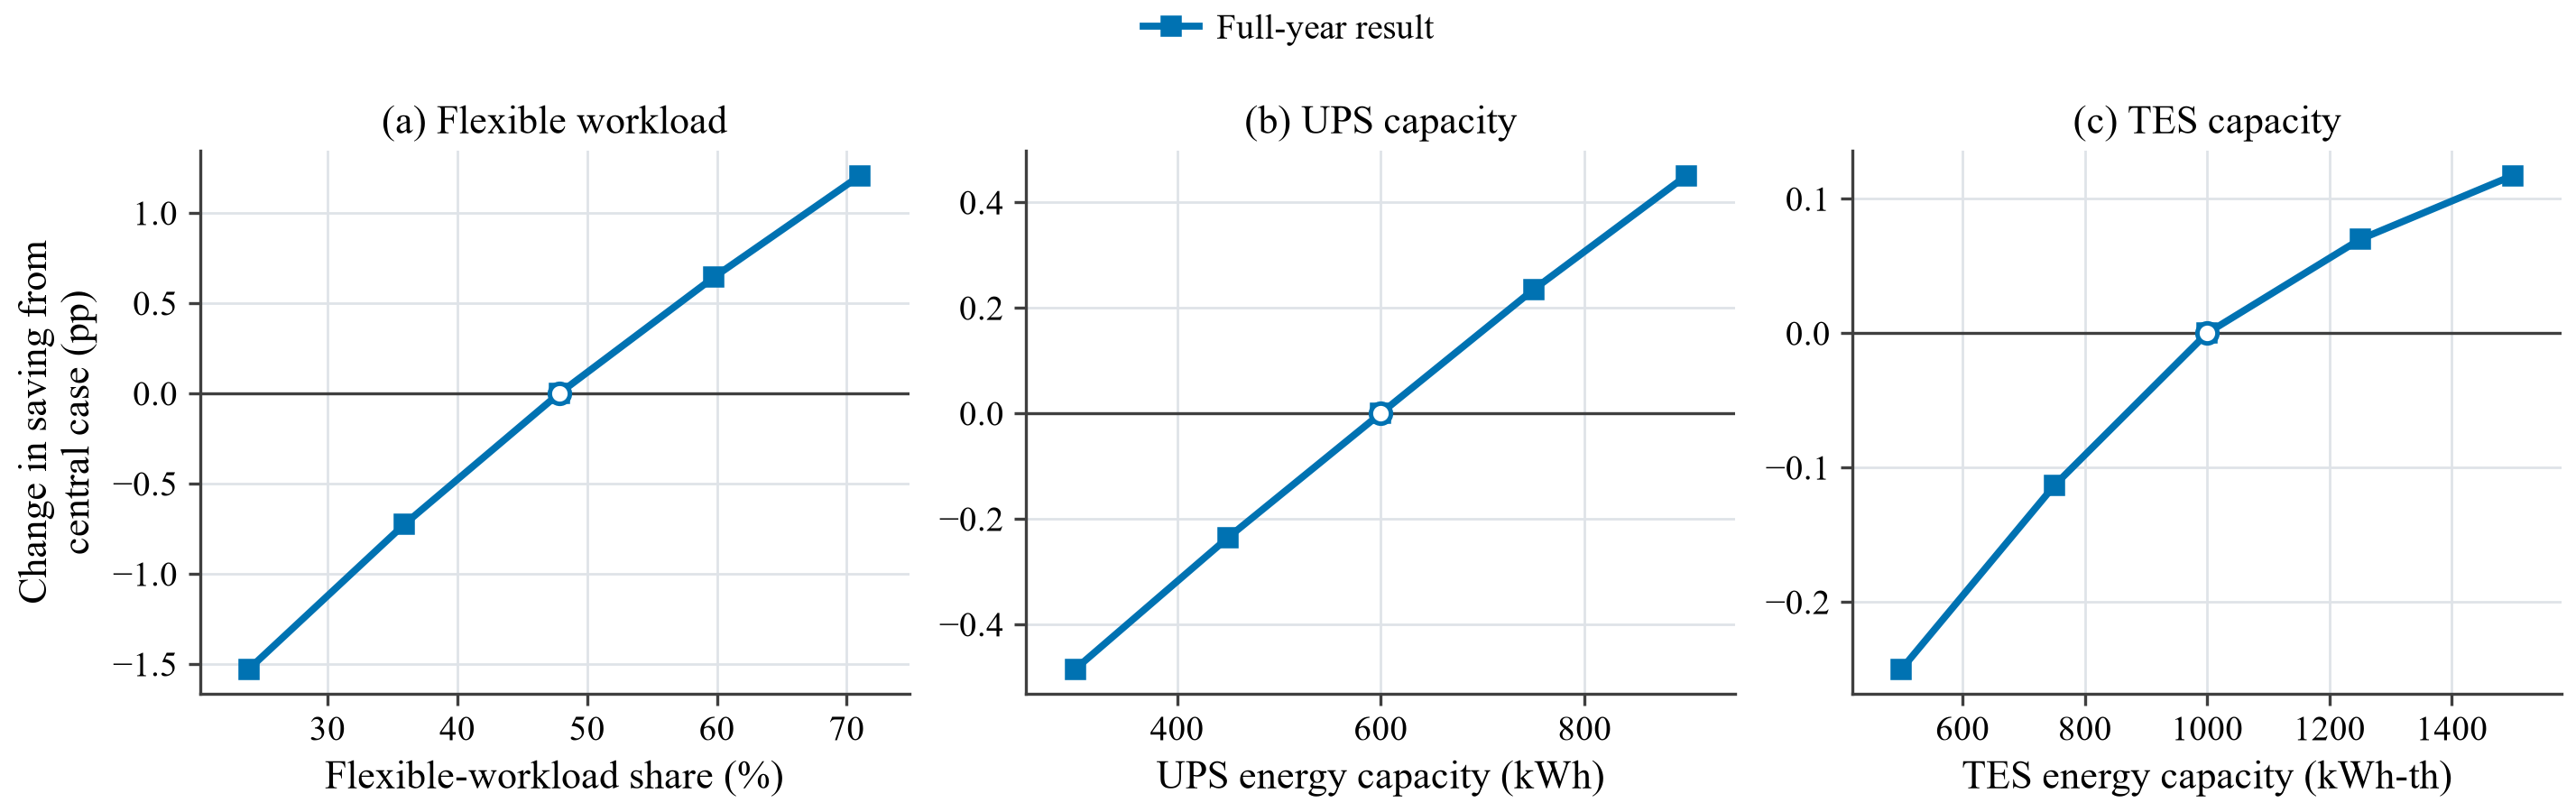
\includegraphics[width=\textwidth]{Figure_9.png}
\caption{Full-year resource sensitivities relative to the central saving, in percentage points. Panel (a) uses the realised flexible share of the daily input CPU-hours after clipping. Note the different vertical scales. Storage power limits remain fixed as energy capacity changes.}
\label{fig:sensitivity}
\end{figure*}

The workload response reflects both the size of IT demand and its link to heat production. Changing eligible workload creates scheduling opportunities throughout the year, whereas extra stored energy remains constrained by charging power, conversion efficiency and opportunities to use it. The smaller TES response is consistent with retaining fixed thermal charge/discharge ratings and a shared chiller limit. Workload-share sensitivity is therefore useful for interpreting a context-dependent assumption; TES sensitivity shows that a larger energy buffer alone does not remove the other constraints on cooling operation.

UPS enlargement poses a more direct design question: how much additional expenditure could its additional operational saving support? Increasing capacity from 600 to 750 kWh reduces annual coordinated cost by GBP~1,292.28. Increasing it to 900 kWh reduces cost by GBP~2,481.41. These increments correspond to GBP~8.62 and GBP~8.27 per added nameplate kWh per year. The second 150 kWh increment is worth less than the first, although the taper is modest. Because the reserve fraction remains 50\%, these additions increase the operational energy window by only 75 and 150 kWh, respectively.

\begin{table}[htbp]
\centering\small
\caption{UPS enlargement screen: constant annual benefit, ten years, 8\% real discount rate and no additional non-electricity costs.}\label{tab:ups-screen}
\begin{tabular}{@{}rrrr@{}}\toprule
Capacity & Added energy & Added saving & Break-even\\(kWh) & (kWh) & (GBP/year) & investment (GBP) \\\midrule
750 & 150 & 1,292.28 & 8,671 \\
900 & 300 & 2,481.41 & 16,650 \\
\bottomrule\end{tabular}
\end{table}


Under the illustrative ten-year, 8\% real-discount assumptions, Table~\ref{tab:ups-screen} gives supported incremental investments of approximately GBP~8,671 and GBP~16,650, equivalent to GBP~57.81 and GBP~55.50 per added nameplate kWh. These are break-even expenditure thresholds, not estimates of installed battery prices. They identify the amount available to cover enlargement if the observed annual savings persisted. Additional installation and operating costs must fit within that amount for the screen to be favourable.

This result gives a bounded interpretation of flexibility-oriented UPS design. The existing energy-arbitrage benefit supplies a contribution towards larger capacity, but the analysis does not establish that enlargement pays for itself. A deployment decision would need compatible installed costs, degradation, replacement and reserve requirements. It would also need to distinguish a larger UPS with the modelled proportional reserve from an expansion that keeps absolute backup energy fixed. Initial and terminal stored energy differ between capacities, so the single-year saving is used as a conditional annuity rather than a demonstrated lifetime cash flow. Alternative discount rates and lives are reported in \supp{8}. No hypothetical payment for the physical events is added to the annual saving.

\subsection{Practical interpretation and limitations}
The flexibility results indicate how coordinated assets can alter demand while preserving modelled computational obligations and recovering relative to undisturbed operation. They are useful inputs to a wider grid-service assessment, but they do not establish network benefit on their own. The annual cost-minimising schedule has a higher import peak, and the model contains neither network power flows nor the behaviour of other loads. A service procurer would also need to specify response speed, event frequency, delivery tolerances and availability. Quarter-hour trajectories cannot demonstrate subsecond response performance.

The facility and workloads are deliberately stylised. The repeated daily workload, fixed ambient temperature and fixed COP exclude seasonal and weekly changes in computing demand and cooling conditions. Aggregate CPU-hours do not represent server placement, task dependencies, memory constraints or every SLA. The conservative cooling rule further defines the available thermal operating envelope. These assumptions allow the interaction of the represented resources to be examined, but the resulting durations should not be transferred directly to a different facility or scaled solely by its IT rating. GPU power management, application-specific performance trade-offs and other forms of flexibility are outside the present workload-shifting model.

Economic and physical conclusions also have different scopes. Annual results quantify signed reference-price electricity costs, with conversion losses but without battery degradation, network tariffs or service revenue. They do not measure the total financial value of flexibility. The event study establishes feasible responses on one selected day, not an annual availability distribution. It includes no preconditioning and requires recovery within a fixed allowance, so its results are conditional on those service rules. Finally, numerical feasibility checks do not constitute experimental validation of the aggregate facility. Solver bounds, duration-search qualifications and existing terminal-treatment checks are reported in the supplement so that these numerical limits remain distinct from the model's physical assumptions.

\section{Conclusion}
\label{sec:conclusion}
This paper characterises data-centre flexibility through an integrated representation of IT workload, UPS storage and cooling with TES. The resulting response depends on the requested power deviation, its start time and the operating state inherited by each resource. Including recovery connects event delivery to the facility's subsequent obligations, while component decomposition reveals the internal actions behind the metered response.

For the 1 MW IT-rated case, the representative-day assessment demonstrates a 100 kW import reduction lasting six hours and a 25 kW import increase reaching the twelve-hour assessment cap. The participating resources vary with timing: selected morning reductions are predominantly supplied by UPS discharge, whereas afternoon reductions rely mainly on workload deferral and reduced cooling. These examples show why equipment capacity alone is insufficient to describe available flexibility, and why a whole-facility assessment is needed to capture compensating actions across assets.

Annual coordinated operation reduces electricity cost by GBP~29,626.91, or 5.38\%, under the observed 2025 reference prices. This saving accompanies greater annual electricity use and peak import, demonstrating the importance of distinguishing price value from energy efficiency and network benefit. Flexible workload share produces the largest economic response among the tested assumptions. Enlarging UPS capacity from 600 to 900 kWh adds approximately GBP~2,460/year in savings and supports a conditional investment threshold, rather than an unconditional case for larger batteries.

The findings support describing flexibility as a state-dependent capability with magnitude, duration and recovery conditions. Extending the assessment to varied workloads and weather, explicit degradation and tariffs, and a broader set of event days would support site-specific investment and market-participation decisions. The present results provide the physical and operational basis for those decisions while keeping annual electricity-cost savings separate from unmodelled service revenues.

\section*{Acknowledgements}
This work was supported by the Engineering and Physical Sciences Research Council and the Economic and Social Research Council through the Energy Demand Research Centre (grant EP/Y010078/1).
\section*{CRediT authorship contribution statement}
\textbf{James Day:} Writing -- original draft, Investigation, Methodology, Conceptualization. \textbf{Mehmet T\"urker Takci:} Writing -- original draft, Investigation, Methodology, Conceptualization. \textbf{Meysam Qadrdan:} Writing -- review \& editing, Supervision, Conceptualization.
\section*{Supporting information}
The supplementary document gives the complete formulation, numerical inputs, annual and event procedures, extended results and investment-screen assumptions. The accompanying data files contain the adopted workload profiles and tabulated results.
\bibliographystyle{IEEEtran}
\bibliography{references}
\end{document}
